%%%%%%%%%%%%%%%%%%%%%%%%%%%%%%%%%%%%%%%%%%%%%%%%%%%%%%%%%%%%%%%%%%%%%%%%
%                                                                      %
%     File: Implementation/02_ModelValidation.tex                      %
%     Tex Master: ../Thesis.tex                                        %
%                                                                      %
%%%%%%%%%%%%%%%%%%%%%%%%%%%%%%%%%%%%%%%%%%%%%%%%%%%%%%%%%%%%%%%%%%%%%%%%

% ==============================================================================
\section{Model Validation}
\label{sec:model_validation}

Before incorporating the vehicle and tether models into the real-time controllers developed in Chapter~\ref{chapter:methodology}, their accuracy and validity must be verified against the high-fidelity simulation environment described in Section~\ref{sec:simulation_environment}. This ensures that the simplified analytical formulations adequately capture the dominant physical dynamics while remaining computationally tractable for online execution.

\subsection{USV Dynamics Validation}
\label{subsec:usv_validation}

The three-degree-of-freedom planar dynamic model derived in Section~\ref{subsec:mod_usv_dynamics} and the thruster allocation described in Section~\ref{subsec:mod_usv_thruster_allocation} provide the predictive backbone for the \gls{usv} trajectory tracking controllers. This control-oriented model intentionally simplifies the physical system by neglecting out-of-plane heave, pitch, and roll motions, as well as wave-induced radiation and diffraction forces. Before embedding this formulation into the real-time optimization loop of the non-linear predictive controller, its ability to reproduce the vessel's planar motions must be verified against the full six-degree-of-freedom physics of the Gazebo simulator.

Rather than relying on empirical grey-box fitting or tuning arbitrary parameters against experimental data, the validation is conducted strictly using the first-principles nominal parameters of the simulation environment. The total vessel mass is set to $m = 259.10\,\text{kg}$, comprising the $227.0\,\text{kg}$ catamaran hull, the two $15.0\,\text{kg}$ stern thruster assemblies, and $2.1\,\text{kg}$ of sensors and propeller pods. The yaw moment of inertia about the centre of gravity is $I_z = 695.90\,\text{kg}\cdot\text{m}^2$, obtained by combining the base hull inertia of $495.0\,\text{kg}\cdot\text{m}^2$ with the parallel axis theorem contribution of the two outboard thrusters mounted at longitudinal distance $x_{\mathrm{arm}} = 2.3738\,\text{m}$ and lateral distance $y_{\mathrm{arm}} = 1.0271\,\text{m}$. The hydrodynamic drag parameters are adopted directly from the simulator configuration given in Table~\ref{tab:usv_damping_parameters}, with linear and quadratic surge damping of $X_u = 100.0\,\text{N}/(\text{m/s})$ and $X_{uu} = 150.0\,\text{N}/(\text{m/s})^2$, sway damping of $Y_v = 100.0\,\text{N}/(\text{m/s})$ and $Y_{vv} = 100.0\,\text{N}/(\text{m/s})^2$, and yaw damping of $N_r = 800.0\,\text{N}\cdot\text{m}/(\text{rad/s})$ and $N_{rr} = 800.0\,\text{N}\cdot\text{m}/(\text{rad/s})^2$.

To excite the full operating envelope of the vessel, a dynamic manual joystick maneuver was recorded in the simulator over $63.84\,\text{s}$, covering a total traversed distance of $61.29\,\text{m}$. The telemetry records the physical actuator commands dispatched to the port and starboard azimuth thrusters, shown in Figure~\ref{fig:usv_actuator_inputs}. The commanded thrust spans the full bidirectional range, reaching the forward saturation limit of $+510.0\,\text{N}$ and the reverse limit of $-380.0\,\text{N}$, while the azimuth angles rotate dynamically up to $\pm 24^\circ$.

\begin{figure}[!htbp]
    \centering
    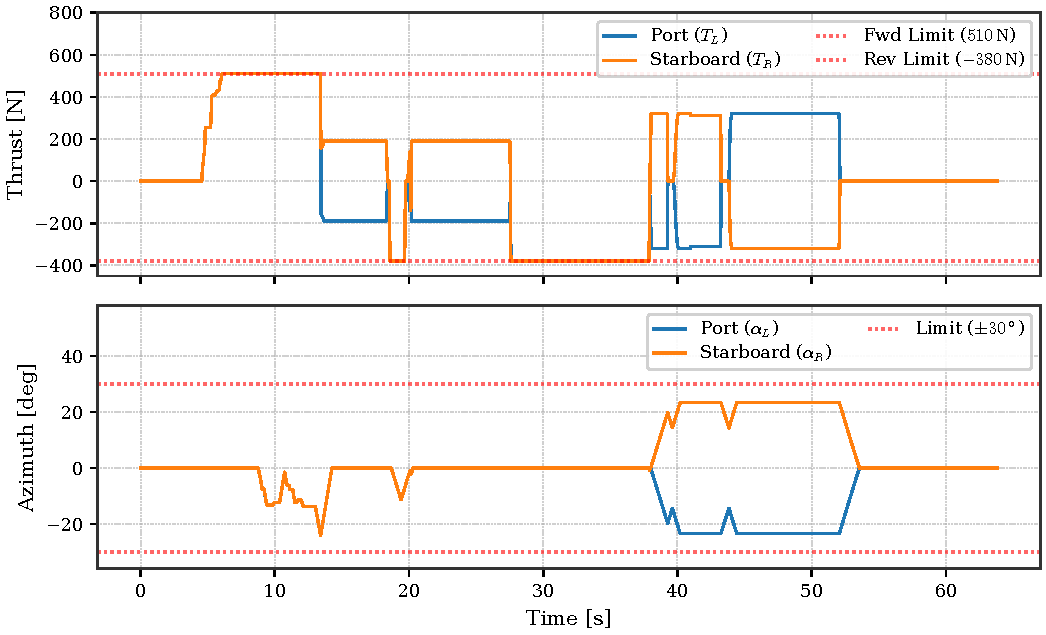
\includegraphics[width=0.75\textwidth]{Implementation/figures/02_model_validation/usv_actuator_inputs.pdf}
    \caption{USV thruster inputs during the validation maneuver.}
    \label{fig:usv_actuator_inputs}
\end{figure}

The nominal model was integrated purely open-loop using a fourth-order Runge-Kutta scheme at $50\,\text{Hz}$, driven exclusively by the actuator commands mapped through equations~\eqref{eq:usv_thruster_force_sum} and~\eqref{eq:usv_thruster_moment}. Figure~\ref{fig:usv_velocities_validation} compares the predicted body-fixed velocities against the ground-truth telemetry from the simulator. The surge velocity $u$ follows the sharp accelerations, cruising phases, and aggressive reverse braking transitions with high fidelity, achieving a coefficient of determination of $R^2 = 99.90\%$ and an \gls{rmse} of $0.0350\,\text{m/s}$. The sway velocity $v$, induced by the lateral components of the angled thrusters, is captured with $R^2 = 99.77\%$ and an \gls{rmse} of $0.0284\,\text{m/s}$. The yaw rate $r$ reproduces both transient steering peaks and sustained rotations, yielding $R^2 = 98.94\%$ and an \gls{rmse} of $0.9925^\circ/\text{s}$.

\begin{figure}[!htbp]
    \centering
    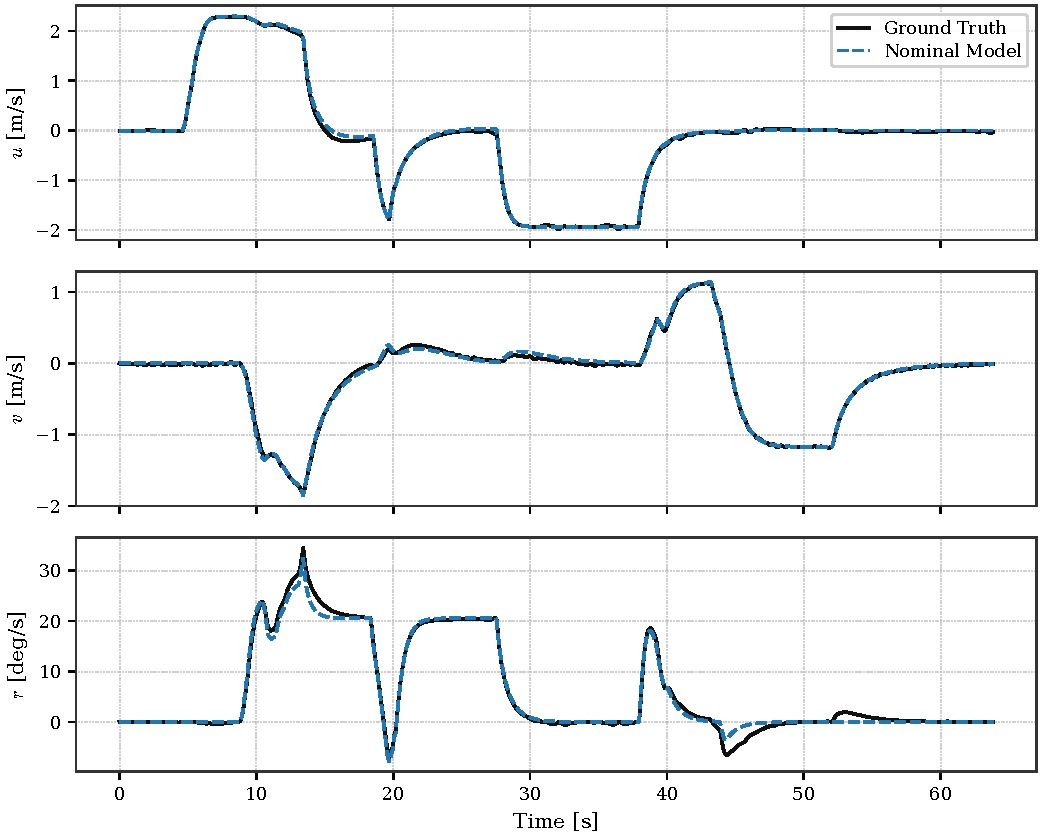
\includegraphics[width=0.75\textwidth]{Implementation/figures/02_model_validation/usv_velocities_validation.pdf}
    \caption{USV body-fixed velocities validation.}
    \label{fig:usv_velocities_validation}
\end{figure}

The kinematic validity of the planar model over extended horizons is demonstrated in Figure~\ref{fig:usv_trajectory_validation}. Over the entire $63.84\,\text{s}$ run, the predicted vessel heading $\psi$ remains tightly aligned with the simulated catamaran, obtaining an $R^2$ of $99.78\%$ and an \gls{rmse} of $7.0173^\circ$. In the horizontal plane, the cumulative Euclidean position error between the open-loop integration and the ground truth reaches an \gls{rmse} of $2.190\,\text{m}$, which corresponds to only $3.57\%$ of the total distance traveled. This small divergence is attributed to unmodeled wave-induced roll and pitch perturbations and the absence of any feedback correction during the open-loop simulation.

\begin{figure}[!htbp]
    \centering
    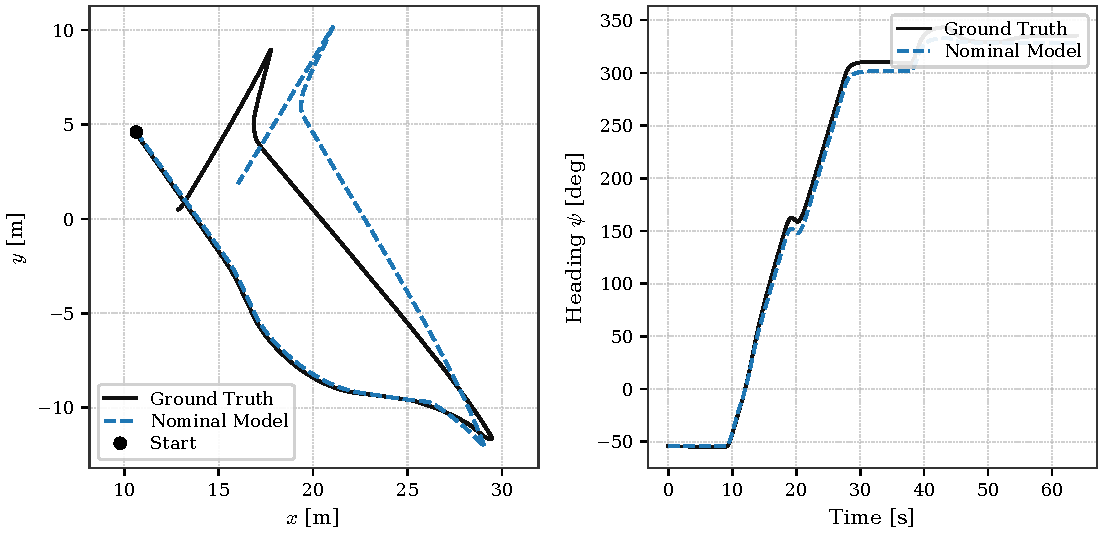
\includegraphics[width=0.82\textwidth]{Implementation/figures/02_model_validation/usv_trajectory_validation.pdf}
    \caption{USV trajectory and heading validation.}
    \label{fig:usv_trajectory_validation}
\end{figure}

Table~\ref{tab:usv_validation_metrics} provides a quantitative summary of the validation metrics across all state variables. The close agreement across all velocity and kinematic states confirms that the first-principles 3-DOF formulation and its thruster allocation equations capture the vessel dynamics with sufficient accuracy for model-based predictive control, without requiring grey-box parameter estimation.

\begin{table}[!htbp]
    \centering
    \caption{USV open-loop model validation metrics.}
    \label{tab:usv_validation_metrics}
    \begin{tabular}{lccccc}
        \toprule
        \textbf{State} & \textbf{Unit} & \textbf{RMSE} & \textbf{MAE} & \textbf{$R^2$ (\%)} & \textbf{Max Error} \\
        \midrule
        Surge velocity $u$ & $\text{m/s}$ & $0.0350$ & $0.0235$ & $99.90$ & $0.1372$ \\
        Sway velocity $v$ & $\text{m/s}$ & $0.0284$ & $0.0217$ & $99.77$ & $0.1010$ \\
        Yaw rate $r$ & $\text{deg/s}$ & $0.9925$ & $0.5989$ & $98.94$ & $3.5991$ \\
        Heading $\psi$ & $\text{deg}$ & $7.0173$ & $5.8392$ & $99.78$ & $11.0267$ \\
        Longitudinal position $x$ & $\text{m}$ & $1.9996$ & $1.4632$ & $89.65$ & $3.2867$ \\
        Lateral position $y$ & $\text{m}$ & $0.8926$ & $0.6802$ & $98.17$ & $1.3779$ \\
        \midrule
        Euclidean position $e_p$ & $\text{m}$ & $2.1901$ & $1.6575$ & -- & $3.4990$ \\
        \bottomrule
    \end{tabular}
\end{table}


\subsection{UAV Inner-Loop Dynamics Validation}
\label{subsec:uav_validation}
% Attitude response and verification of the inner-loop attitude lag (tau = 0.15 s)

\subsection{Tether Model Validation}
\label{subsec:tether_model_validation}

The control architecture developed in Chapter~\ref{chapter:methodology} requires an estimate of the three-dimensional force $\mathbf{F}_{\mathrm{tether}}^{\mathcal{I}}$ exerted by the cable on the \gls{uav} to compensate for tether coupling and enforce tension constraints. In simulation, the cable is represented by a high-fidelity lumped-mass model in MoorDyn, which captures multi-node elasticity, bending stiffness, and hydrodynamic drag. However, evaluating such a high-degree-of-freedom representation or solving the non-linear catenary boundary value problem numerically at every control cycle or across the prediction horizon of an \gls{mpc} is computationally prohibitive. A closed-form, control-oriented model is therefore essential to provide instantaneous force predictions with negligible computational overhead.

The first-principles formulation derived in Section~\ref{subsec:mod_tether_force_model} computes the tether force directly from its nominal physical specifications under steady winch regulation. With the winch maintaining the slack ratio around $\varepsilon_0 = 0.05$, the linear mass density $\mu = 0.020\,\text{kg/m}$ and gravitational acceleration $g = 9.81\,\text{m/s}^2$ yield a nominal tension-distance coefficient of
\begin{equation}
    c_d(\varepsilon_0) = \frac{\mu\,g}{1 - \varepsilon_0} = \frac{0.020 \times 9.81}{1 - 0.05} \approx 0.2065\,\text{N/m},
    \label{eq:tether_val_cd}
\end{equation}
giving the scalar tension estimate $T_{\mathrm{theo}}(d) = c_d(\varepsilon_0)\,d$, where $d = \|\mathbf{p}_v - \mathbf{p}\|$ is the Euclidean distance between the \gls{usv} and the \gls{uav}. In terms of the unstretched cable length $L$, this corresponds to $T_{\mathrm{theo}}(L) = \mu\,g\,L = 0.1962\,L$. The three-dimensional direction $\hat{\mathbf{d}}$ is constructed by tilting the line-of-sight chord $\hat{\mathbf{d}}_0$ towards the vertical by the nominal catenary elevation deflection angle $\gamma(\alpha) = \gamma_0\cos\alpha$, where $\gamma_0 = 28.0^\circ$ is the nominal deflection at $\varepsilon_0 = 0.05$ and $\alpha$ is the chord depression angle. To assess whether this nominal model adequately captures the coupling dynamics, its predictions are evaluated against telemetry from the 30-segment MoorDyn simulator recorded during a $60.5\,\text{s}$ flight trajectory with separation distances ranging from $4.6\,\text{m}$ to $14.0\,\text{m}$. Furthermore, the formulation is benchmarked against two widespread simplifications from the tethered multirotor literature.
\begin{enumerate}
    \item \textbf{Pure Vertical Ballast}, which assumes that the tether hangs directly downward as an equivalent vertical load with $\mathbf{F}_{\mathrm{pure\_z}} = [0,\,0,\,-T_{\mathrm{theo}}]^T$, neglecting horizontal coupling.
    \item \textbf{Pointing to \gls{usv} (Straight Chord)}, which assumes a taut cable between the attachment points with $\gamma = 0^\circ$, directing the full tension along the direct line of sight with $\mathbf{F}_{\mathrm{chord}} = T_{\mathrm{theo}}\,\hat{\mathbf{d}}_0$.
\end{enumerate}

Figure~\ref{fig:model_fit_comparison} compares the predicted scalar tension magnitude $T_{\mathrm{theo}}(t)$ with the filtered MoorDyn telemetry over the trajectory. The theoretical linear relation with $c_d = 0.2065\,\text{N/m}$ follows the actual tension closely across the entire operating range, achieving a coefficient of determination of $R^2 = 91.2\%$ and an \gls{rmse} of $0.2031\,\text{N}$.

\begin{figure}[!htbp]
    \centering
    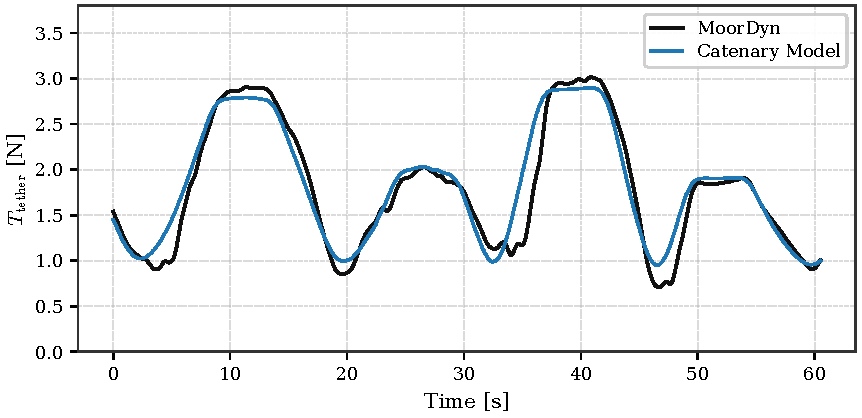
\includegraphics[width=0.75\textwidth]{Implementation/figures/02_model_validation/model_fit_comparison.pdf}
    \caption{Tether tension magnitude at the \gls{uav}.}
    \label{fig:model_fit_comparison}
\end{figure}

When resolved into Cartesian components in the inertial frame in Figure~\ref{fig:model_fit_3d}, the importance of accounting for the catenary deflection angle $\gamma_0 = 28.0^\circ$ becomes evident. The proposed formulation accurately tracks both the horizontal restoring force $F_x$ with $R^2 = 97.6\%$ and $\text{RMSE} = 0.1457\,\text{N}$, as well as the vertical downward pull $F_z$ with $R^2 = 86.9\%$ and $\text{RMSE} = 0.2339\,\text{N}$. In contrast, the pure vertical simplification fails completely to capture horizontal interaction forces with $R^2 = -0.7\%$, while the straight chord approximation directs excess tension into the horizontal axis and underestimates vertical load because it ignores the natural sag of the cable.

\begin{figure}[!htbp]
    \centering
    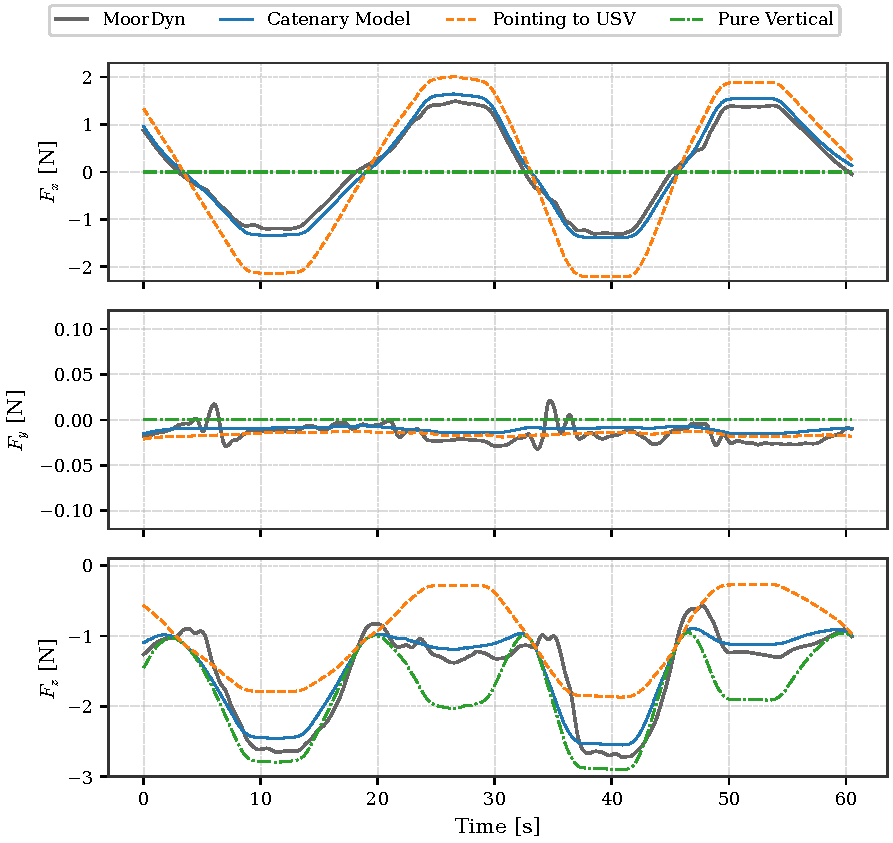
\includegraphics[width=0.82\textwidth]{Implementation/figures/02_model_validation/model_fit_3d_components.pdf}
    \caption{Three-dimensional tether force components at the \gls{uav}.}
    \label{fig:model_fit_3d}
\end{figure}

The temporal evolution of the three-dimensional prediction error norm $\|\mathbf{F}_{\mathrm{true}} - \mathbf{F}_{\mathrm{model}}\|$, presented in Figure~\ref{fig:model_fit_residuals}, reveals the stability of each approach during dynamic manoeuvres. While the baseline simplifications experience large transient error surges exceeding $1.6\,\text{N}$ during vehicle reversals, the proposed catenary model maintains a low and bounded residual below $0.4\,\text{N}$ throughout the entire flight profile.

\begin{figure}[!htbp]
    \centering
    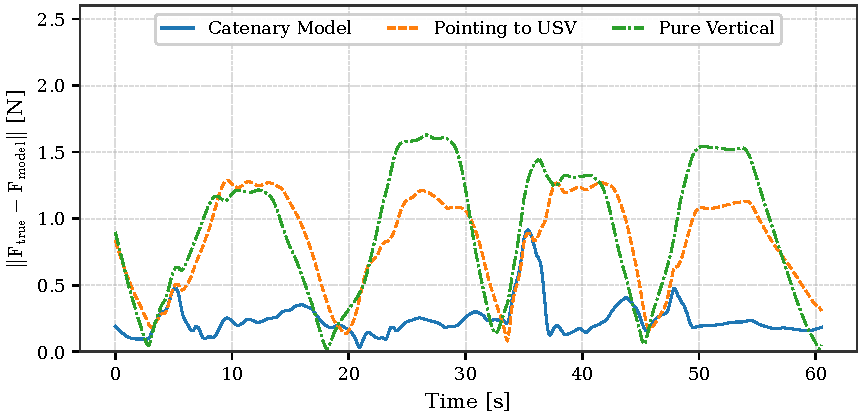
\includegraphics[width=0.75\textwidth]{Implementation/figures/02_model_validation/model_fit_residuals.pdf}
    \caption{Three-dimensional tether force error norm.}
    \label{fig:model_fit_residuals}
\end{figure}

Table~\ref{tab:tether_model_benchmark} summarises the quantitative performance across the complete benchmark trajectory. The proposed first-principles model achieves an overall three-dimensional \gls{rmse} of $0.2757\,\text{N}$, reducing the spatial force error by more than $70\%$ compared to both the straight chord model with $0.8991\,\text{N}$ ($+226.1\%$ error) and the pure vertical model with $1.0332\,\text{N}$ ($+274.7\%$ error). These results confirm that the closed-form catenary approximation captures the dominant coupling forces with sufficient fidelity for real-time feedforward compensation, while avoiding the prohibitive computational cost of numerical catenary solvers or multi-segment models.

\begin{table}[!htbp]
    \centering
    \caption{Tether force model benchmark.}
    \label{tab:tether_model_benchmark}
    \begin{tabular}{lcccccc}
        \toprule
        \textbf{Model} & \textbf{$F_x$ $R^2$} & \textbf{$F_x$ RMSE} & \textbf{$F_z$ $R^2$} & \textbf{$F_z$ RMSE} & \textbf{3D RMSE} & \textbf{Error Increase} \\
        & (\%) & (N) & (\%) & (N) & (N) & \\
        \midrule
        \textbf{Proposed Catenary} & $\mathbf{97.6}$ & $\mathbf{0.1457}$ & $\mathbf{86.9}$ & $\mathbf{0.2339}$ & $\mathbf{0.2757}$ & \textbf{Baseline} \\
        Pointing to \gls{usv} ($\gamma = 0^\circ$) & $57.4$ & $0.6135$ & $-3.8$ & $0.6572$ & $0.8991$ & $+226.1\%$ \\
        Pure Vertical ($F_z = -T$) & $-0.7$ & $0.9438$ & $57.6$ & $0.4200$ & $1.0332$ & $+274.7\%$ \\
        \bottomrule
    \end{tabular}
\end{table}
